\section{Experiments}
\label{sec:exp}
\subsection{Data Preparation}
\label{sec:exp:prep}

\vpara{Dataset.}
% years

We prepared several representative datasets for the variables we need: $\EFF$, $\HFF$, and $\FFF$.
\vpara{Fragility Score Index.}

\vpara{Environmental Performance Index.}

\vpara{Other Indicators.}

\subsection{Calculation of Fragility Score}
In order to calculate fragility score defined in Section~\ref{sec:model:frag}, we need to identify, a priori, which states are fragile and which states are environmentally unstable. 
In order to achieve so, we determine that a state is fragile, i.e. $\FFF=1$, if its FSI score is higher than a certain threshold $F_0$, and a state is environmentally fragile, i.e. $\EFF=1$, if its EPI score is lower than a certain threshold $E_0$. 
The thresholds are chosen differently for each year, because the indexes of different years aren't necessarily calculated using the same methodology.
Therefore, thresholds for each year are chosen to guarantee that the fragile states and environmentally fragile states occupy approximately $30\%$ of the states, respectively. As such, each state's status of fragility and environmental fragility is approximated by HSI and EPI indexes. Furthermore, we use the 12 indicators used in the calculation of FSI, specified in \reminder{specify somewhere}, as components of human factors $\HFF = \left[ h_1\ldots h_12 \right]$.

Hence, all variables needed for the calculation of our fragility score, including $\HFF, \EFF, \FFF$, are specified for each state. Logistic regression was run as described in Section~\ref{sec:model:frag} to obtain fragility score of each state. Finally, we visualize the relationship between the score and the two indexes in Figure~\ref{fig:exp:frag_relation}.

\begin{figure}[htbp]
   \caption{Relationship between Fragility Score $\FFS$ and FSI and EPI.} 
   \label{fig:exp:frag_relation}
\end{figure}

\subsection{Direct Effect of Environmental Factors}
\label{sec:exp:direct}

\begin{figure}[htbp]
    \centering
    \subfigure[General Effect] {
        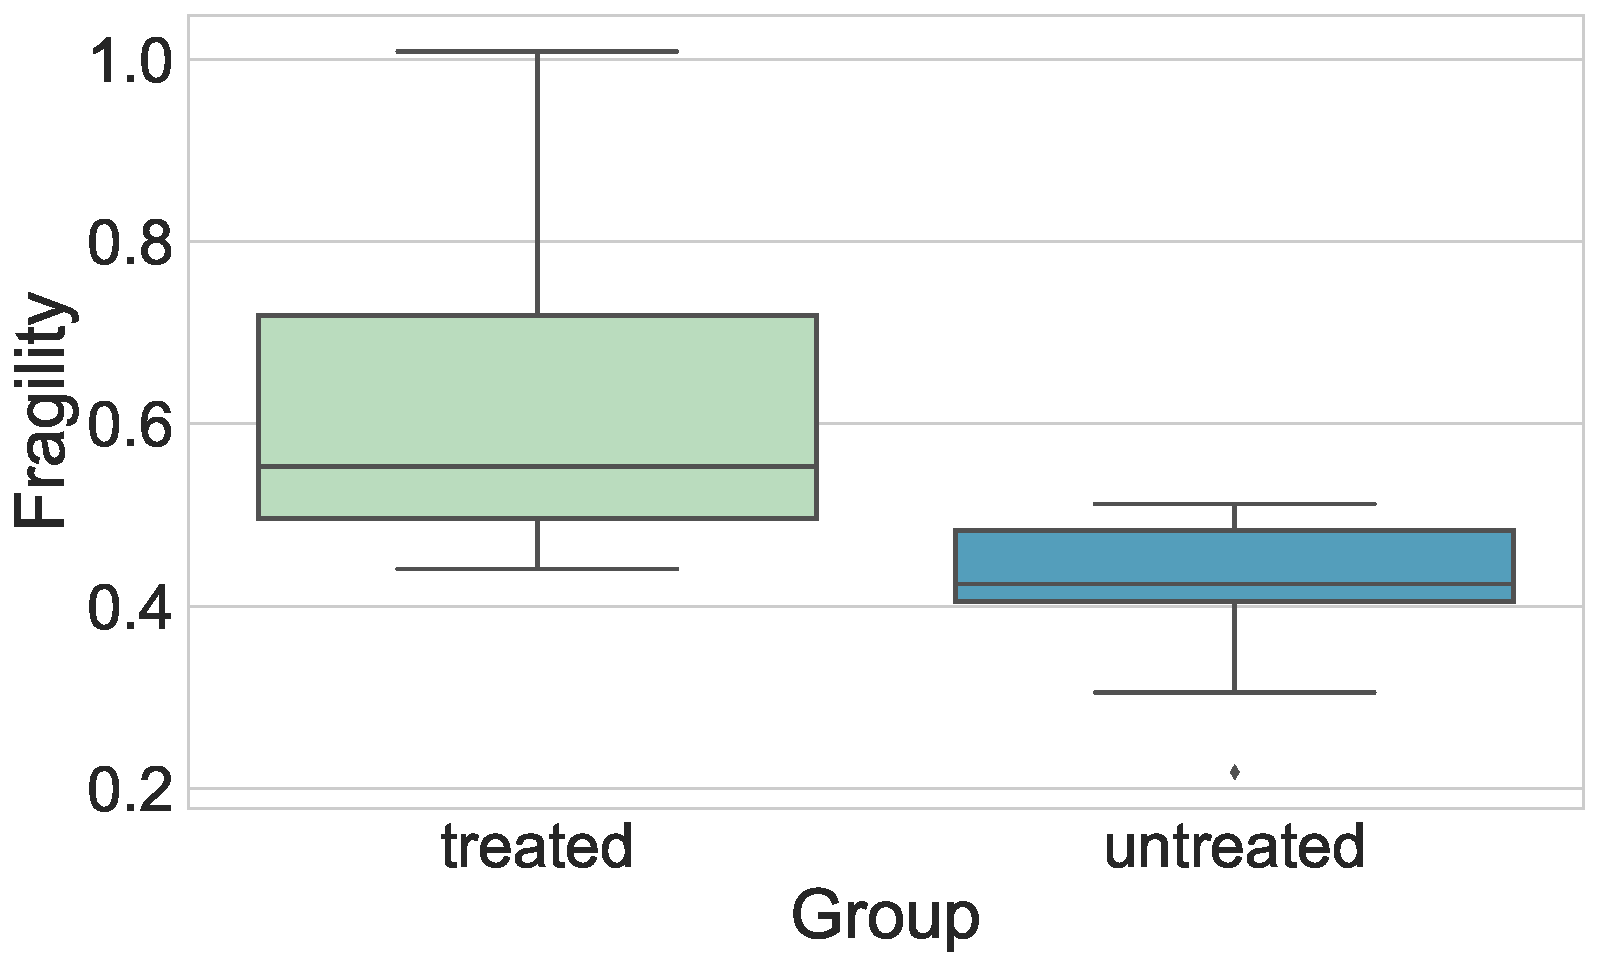
\includegraphics[width=.48\linewidth]{figs/fragility_treat}
        \label{fig:exp:direct:general}
    }
    \subfigure[Specific Countries] {
        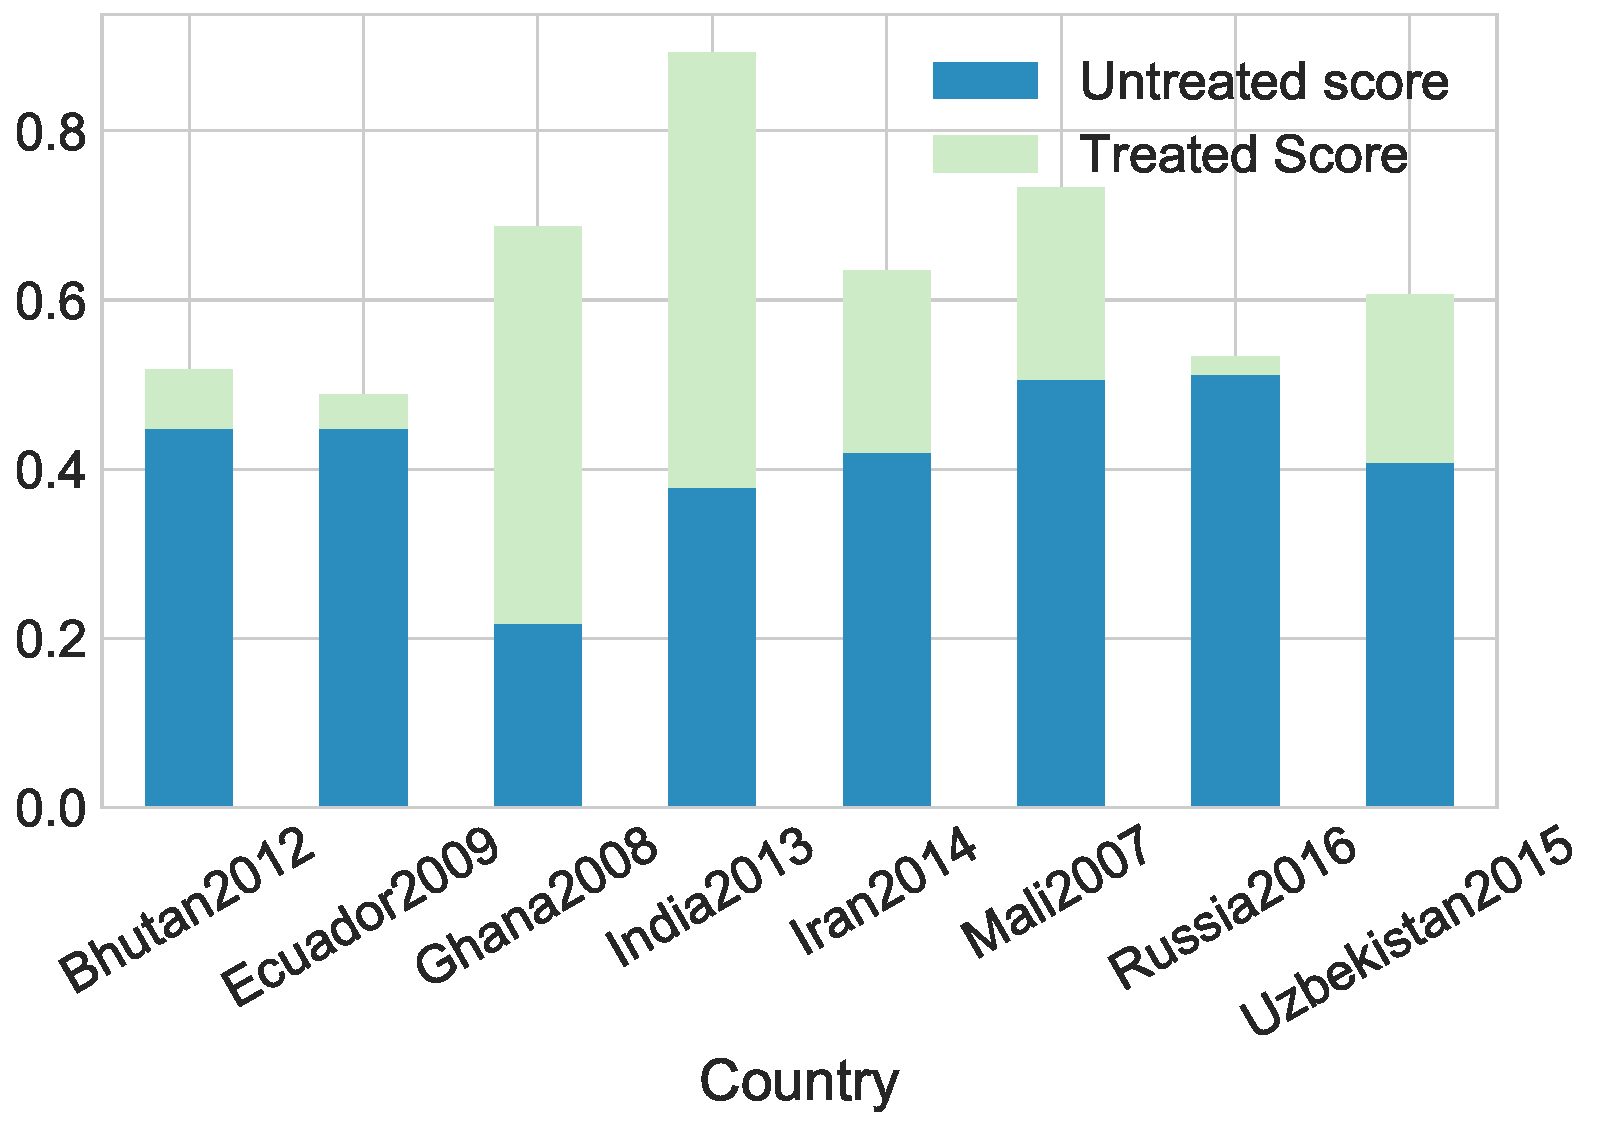
\includegraphics[width=.48\linewidth]{figs/compare_score}
        \label{fig:exp:direct:specific}
    }
    \caption{Direct Effect of Environmental Factors.}
\end{figure}

\subsection{Indirect Effect of Environmental Factors}

To measure the indirect effect of environmental factors, we modeled several regression models in Section~\ref{sec:model:indirect}. Specifically, we choose the EPI index and FSI index described in Section~\ref{sec:exp:prep} to represent the environmental factors $\EFF$ and human factors $\HFF$, respectively. The indexes are scaled and centralized, such that a comparsion of coefficients is meaningful.
\begin{table}[htbp]
    \centering
   \begin{tabular}{|l|ccc|} \hline
      Variable & $\EFF$ & $\HFF$ & $\EFF\times\HFF$ \\ \hline
      Coefficient & 0.17 & 0.91 & 0.06 \\ \hline
      P-value & 0.31 & 0.00 & 0.69679 \\ \hline
      Significant & No & Yes & No  \\ \hline
   \end{tabular} 
   \caption{Moderator variable model of human factors.}
   \label{tab:exp:moderator}
\end{table}

\vpara{Moderator Effect.}
The regression parameters and their p-value is listed in Table~\ref{tab:exp:moderator}. Lower p-value indicates that the original hypothesis that was tested is insignificant. We determine that if the p-value lower a certain threshold, $0.05$, we would reject the hypothesis. Since our hypothesis detailed in Section~\ref{sec:model:indirect} is that the coefficient is zero, p-value lower than $0.05$ would show that the effect of the corresponding variable is significant.

Table~\ref{tab:exp:moderator} shows that the moderator effect is not significant; therefore we would reject the hypothesis that the human factors act as a moderator of the relation between the environmental factors and the fragility.

\begin{table}[htbp]
    \centering
    \begin{tabular}{|l|cccc|} \hline
        Variable & Model & Coef. & p-val. & Sign.  \\ \hline
        % \multirow{2}{*}{Human factors} & $\FFF\sim\HFF$ & -0.8349 & $<2e-16$ & Yes \\ \cline{2-5}
        Human factors & $\FFF\sim\HFF + \EFF$ & 1.009 & $<2e-16$ & Yes  \\ \hline        
        \multirow{3}{*}{Environmental factors} & $\HFF\sim\EFF$ & -0.8349 & $<2e-16$ & Yes \\ \cline{2-5}
        & $\FFF\sim\EFF$ & -0.6152 & $<2e-16$ & Yes \\ \cline{2-5}
        & $\FFF\sim\HFF+\EFF$ & 0.2272 & 0.00773 & Yes \\ \hline        
    \end{tabular}
    \caption{Mediator variable effect of human factors. The column Model tells the regression model, in which the left hand of $\sim$ is the dependent variable, and the right hand are the independent variables used in the regression model.}
    \label{tab:exp:mediator:general}
\end{table}
    
\vpara{Mediator Effect.}
Table~\ref{tab:exp:mediator:general} shows the result of the test of the mediator effect of human factors, represented by the FSI index. The results show that the effect of human factors on fragility is significant, and that the effect of environmental factors on fragility is significant, by corresponding coefficients in models $\FFF\sim\HFF+\EFF$ and $\HFF\sim\EFF$. In both models of $\FFF\sim\EFF$ and $\FFF\sim\HFF+\EFF$, the effects of human factors on the fragility are significant; furthermore, the absolute value of the coefficient is reduced by approximately $0.4$ once $\HFF$ is introduced. Therefore, the human factors act as a mediator variable, through which the environmental factors influence fragility. Furthermore, model $\FFF\sim\EFF$ shows that environmental factors also influence fragility directly. As such, a statistical proof of the mediator variable model in Section~\ref{sec:model:indirect} is complete.

We are also interested in how the influence of environmental factors propagate through human factors. Therefore, we choose the 12 indicators used in the calculation of HSI index~\reminder{citation}, and construct a new regression model: $\FFF\sim\EFF+h_1+\ldots+h_12$, where $h_i$ is an individual factor. However, not all of the indicators are significant, therefore we attempt to find best subset of indicators that are significant by stepwise regression: at each step, we remove from the regression model an indicator that is statistically insignificant. Since previously removed indicator could be significant in the new model, we add at each step a previously removed indicator that has become significant to the regression model, if there is one. We stop when there is no insignificant indicator to remove and no significant indicator to add. 

The used subset of indicators, their coefficients and significance are shown in Table~\ref{tab:exp:mediator:subset}.
Experiments show that the impact of environmental change propagates mainly through demographic pressures, human flight and brain drain, and human rights. It also flows through group grievance in a less significant manner. Furthermore, it goes through Economy and refugee flows slightly. 

\begin{table}[htbp]
   \centering 
   \begin{tabular}{|l|ccc|} \hline
      Variable & Coef. & p-value & Sign. \\ \hline 
       DP & 0.3009 & 0.00691 & High \\ \hline
       HFBD & 0.2579 & 0.00287 & High \\ \hline
       HR & 0.2424 & 0.00196 & High \\ \hline
       GG & 0.1643 & 0.01824 & Medium \\ \hline
       Econ. & 0.1380 & 0.08155 & Low \\ \hline
       RI & 0.1275 & 0.08768 & Low \\ \hline
   \end{tabular}
   \caption{Best subset of mediator indicators. Rows are respectively: Demographic Pressures, Human Flight and Brain Drain, Human Rights, Group Grievance, Economy, and Refugees and IDPs.}
   \label{tab:exp:mediator:subset}
\end{table}

\vpara{Conclusion on Indirect Effects.} Above experiments show that:
\begin{itemize}
   \item The environmental factors and human factors both directly influence fragility;
   \item Environmental factors also influence human factors, and human factors act as a mediator variable to pass the influence of the environmental factors to fragility 
\end{itemize}
Which is illustrated in Figure~\ref{fig:model:indirect:mediator}. 

\subsection{Temporal Model}
\label{sec:exp:temporal}

\subsection{Regional Model}
\label{sec:exp:regional}